\documentclass[
LEEC,			% Use this option to select your DEE degree, options: LEEC, LETI
english,		% Select document language, options: portuguese or english
%draft,	% Uncomment for draft mode (no pictures, no links, overfull hboxes) 
%twocolumn
]{DEEclass}

% Use the 'preamble.tex' file (root folder) do add packages and macros. Keep your main.tex file clean.

% FYI, the following packages are preloaded with the document class:
% longtable, xcolor, graphicx, booktabs, caption, csquotes, hyperref,
% calc, listings, datetime2, siunitx, geometry, enumitem

%%%%%%%%%%%%%%%%%%%%%%%%%%%%%%%%%%%%%%%%%%%%%%%%%%%%%%%%%% extra packages
\usepackage{amsmath}		% the main package in the AMS-LATEX distribution
\usepackage{amsfonts}		% extended set of fonts for use in mathematics
\usepackage{amssymb}		% adds new symbols to be used in math mode
\usepackage{mathrsfs}		% math fonts, e.g., Laplace
\usepackage{float}			% provides the H float modifier option
\usepackage{multirow}		% tables \multirow command
\usepackage{subcaption}		% enables subfigures
\usepackage{lscape}			% for landscape mode
\usepackage{verbatim}		% new verbatim environment, 
\usepackage{multicol}		% enables multicolumns 
\usepackage[intoc, english]{nomencl} % add nomenclature
\makenomenclature
\usepackage{etoolbox}       % used for nomenclature, i guess...
\makeglossaries
\usepackage{wrapfig}        % enable wrapping figures graphics
\usepackage{graphicx}       % enable graphics
\let\cleardoublepage=\clearpage     % delete blank pages
%\begin{comment}...\end{comment}, \verbatiminput


%add extra packages if needed here

%%%%%%%%%%%%%%%%%%%%%%%%%%%%%%%%%%%%%%%%%%%%%%%%%%%%%%%%%% temp packages
\usepackage{lipsum}						% for fake text
%\usepackage[textsize=tiny]{todonotes}   % enable To-do notes, use the option "disable" to hide all notes, usage \todo{}

%\usepackage{draftwatermark}			% prints a watermark overlay, uncomment if needed
%\SetWatermarkText{**DRAFT**}
%\SetWatermarkScale{1}
%\SetWatermarkColor[gray]{0.8}

%%%%%%%%%%%%%%%%%%%%%%%%%%%%%%%%%%%%%%%%%%%%%%%%%%%%%%%%%% settings
\AtBeginDocument{					% Rendered PDF metadata:
\hypersetup{pdftitle=\ttitle} 		% Sets the PDF title to your dissertation title
\hypersetup{pdfauthor=\authorname} 	% Sets the PDF author to your name
}

%%%%%%%%%%%%%%%%%%%%%%%%%%%%%%%%%%%%%%%%%%%%%%%%%%%%%%%%%% user defined macros









	
% \makenomenclature

%%%%%%%%%%%%%%%%%%%%%%%%%%%%%%%% REPORT INFORMATION %%%%%%%%%%%%%%%%%%%%%%%%%%%%%%%%%%%%%

\reporttitle{Mécanique du Vol d'Un Kite} % Your report title

\author{Kite Design}	% Your name
\studentnumber{0673627662}	% Your student number
\studentemail{1234567@isep.ipp.pt}	% Your student email address  

\advisor{Nome do Orientador}{xxx@isep.ipp.pt}	% Your ISEP advisor name and email
\coadvisor{Nome do Coorientador}{xxx@isep.ipp.pt}	% Your ISEP co-advisor name and email, comment this line if not needed
\company{Nome da Empresa, Lda.}	% The company name where you developed your work, comment this line if not needed
\supervisor{Nome do Orientador da Empresa}{xxx@emailaddress.com} % Your company supervisor name, comment this line if not needed

%%%%%%%%%%%%%%%%%%%%%%%%%%%%%%%%%%%%%%%%%%%%%%%%%%%%%%%%%%%%%%%%%%%%%%%%%%%%%%%%%%%%%%%%%
\begin{document}

\printcoverpage

\tableofcontents

%%%%%%%%%%%%%%%%%%%%%%%%%%%%%%%%%%% MAINMATTER %%%%%%%%%%%%%%%%%%%%%%%%%%%%%%%%%%%%%%%%%

\chapter{Introduction}
\label{ch:Ch0}

Ce bureau d'étude a pour sujet l'équilibre du Kite, sa condition d'existence et sa stabilité. L'objectif final étant de déterminer des paramètres optimaux tels que le towpoint.
\include{Chapters/01 - Définitions}
\chapter{\textbf{Equilibre Statique Du Kite}}
\label{ch:Ch2}

\textbf{On utilise un modèle de kite "point masse" pour définir l'équilibre statique.} En effet, comme mentionné dans "Dynamic Model of a Pumping Kite Power System" (fechner, 2015), le modèle plus complexe (mais moins simplificateur) qui consiste à considérer 4 points masses (bouts d'aile, centre du kite, attache du bridage) permet de prendre en compte les phénomènes d'inertie du kite dans le virage et de déformation du kite pour pénaliser sa trainé et son taux de virage. le modèle point masse est donc un bon compromis entre hypothèses simplificatrices et prise en compte des phénomènes prédominants sur l'équilibre du kite au zénith. 

%%%%%%%%%%%%%%%%%%%%%%%%%%%%%%%%%%%% SECTION 1
\section{Approche simplifiée} 
\label{sec:Ch2.1}

\begin{figure}[H]
    \centering
    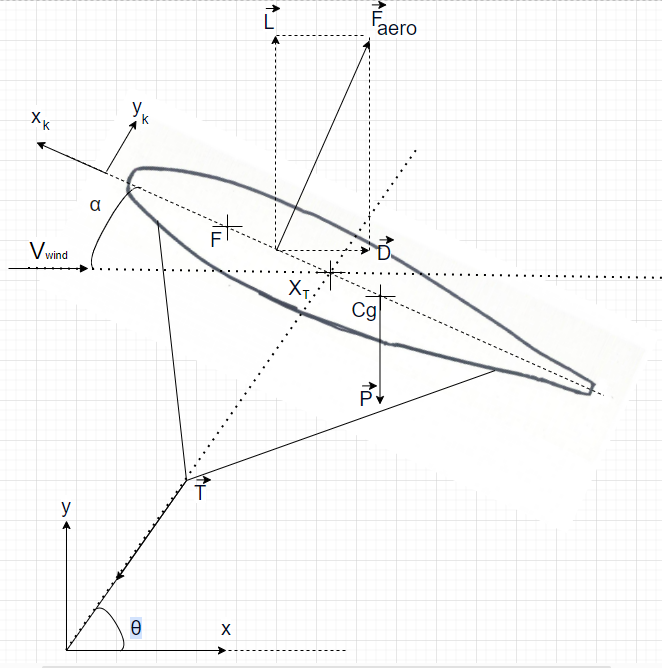
\includegraphics[width=0.5\textwidth]{Pics/02 - Equilibre Statique du Kite/Equilibre Kite.png}  
    \caption{Equilibre du kite}
    \label{fig:Equilibre du kite}
\end{figure}

\textbf{L'angle theta doit être compris comme l'angle que fait le dernier segment de lignes, au point d'attache avec le kite, par rapport à la vertical}. Soit $\theta = \frac{\pi}{2} + \alpha_d - \alpha$ si on se réfère à \ref{fig:fechner alpha d}.\\

Dans le cas particulier où le fardage est négligeable (i.e. trainée des lignes négligeable devant les autres efforts), alors l'angle theta devient celui représenté sur la figure \ref{fig:Equilibre du kite}.

On écrit l'équilibre statique de \{kite+bridage\}, en $X_T$ du kite : 

\begin{equation}
    \begin{cases}
        L = P + T sin(\theta) \\
        D = T cos(\theta) \\
        0 = C_{M_0} + (x_T - x_F) (L cos(\alpha) + D sin(\alpha)) - P cos(\alpha) (x_T - x_G)
    \end{cases}
\end{equation}

Ainsi, en considérant $\alpha << 1$, on a :

\begin{equation}
    \begin{cases}
    \frac{L-P}{D} = tan(\theta) \\
    \theta = \frac{\pi}{2} - \alpha + \alpha_d \\
    x_T = \frac{L x_F - P x_G -C_{M_0}}{L - P}
    \end{cases}
    \label{eq:Xt}
\end{equation}
    
Il semblerait donc que le calcul (CFD, VSM, ...) des polaires aérodynamiques ($L(\alpha)$ et $D(\alpha)$) permettent de trouver le $X_T$ optimal afin d'optimiser la finesse au zénith. 

\textit{Exemple : }
Pour $\alpha_{optimal} = 21^\circ$, $C_D = 0.19$ et $C_L = 1.35$, on trouve en appliquant l'équation \ref{eq:Xt} : \\

\begin{equation}
    \begin{cases}
    \alpha_d =  -12^\circ\\
    \theta = 81^\circ\\
    x_T = 0.22
    \end{cases}
    \label{eq:Xt results}
\end{equation}

avec $P = 21 kg$, $x_F = 0.25$, $x_G = 0.5$,$\frac{1}{2} \rho S v^2 = \frac{1}{2} 1.225 * (50m^2) * (14 * 0.514 m/s)^2$  et $C_{M_0} = 0$ \\

De plus, avec  $d = \frac{6.9 m}{4.56 m} = 1.51 m$ pour une $50m^2$ (d'après SurfPlan). On a finalement :\\
$x_{TP} = -0.10 $

Ce resultat semble correct en ordre de grandeur (comme celui de $x_{TP}$) mais pas "exacte"; comparé aux observations expérimentales. On comprend donc l'importance de déterminer chaque grandeur, notamment les coefficients aérodynamiques, avec davantage de précision !

%%%%%%%%%%%%%%%%%%%%%%%%%%%%%%%%%%%% SECTION 2
\section{Principe Fondamental de la Statique} 
\label{sec:Ch2.2}

\textbf{On souhaite désormais effectuer le calcul rigoureux de l'équilibre du système \{kite, bridage, lignes\}}.




%%%%%%%%%%%%%%%%%%%%%%%%%%%%%%%%%%%% SECTION 3
\section{\textbf{Condition d'existence de l'équilibre du kite}} 
\label{sec:Ch2.3}

\subsection{Angle d'élévation minimal} 
\label{sec:Ch2.3.1}

\subsection{Angle d'élévation maximal}
\label{sec:Ch2.3.2}


%%%%%%%%%%%%%%%%%%%%%%%%%%%%%%%%%%%% SECTION 4
\section{\textbf{Stabilité du kite}} 
\label{sec:Ch2.4}


%%%%%%%%%%%%%%%%%%%%%%%%%%%%%%%%%%%%%%%%%%%%%%%%%%%%%%%%%%%%%%%%%%%%%%%%%%%%%%%%%%%%%%%%% BIBLIOGRAPHY


\end{document}